% !TEX TS-program = pdflatex
% !TEX encoding = UTF-8 Unicode

% This is a simple template for a LaTeX document using the "article" class.
% See "book", "report", "letter" for other types of document.

\documentclass[11pt]{article} % use larger type; default would be 10pt

\usepackage[utf8]{inputenc} % set input encoding (not needed with XeLaTeX)

%%% Examples of Article customizations
% These packages are optional, depending whether you want the features they provide.
% See the LaTeX Companion or other references for full information.

%%% PAGE DIMENSIONS
\usepackage{geometry} % to change the page dimensions
\geometry{a4paper} % or letterpaper (US) or a5paper or....
% \geometry{margin=2in} % for example, change the margins to 2 inches all round
% \geometry{landscape} % set up the page for landscape
%   read geometry.pdf for detailed page layout information

\usepackage{graphicx} % support the \includegraphics command and options

% \usepackage[parfill]{parskip} % Activate to begin paragraphs with an empty line rather than an indent

%%% PACKAGES
\usepackage{booktabs} % for much better looking tables
\usepackage{array} % for better arrays (eg matrices) in maths
\usepackage{paralist} % very flexible & customisable lists (eg. enumerate/itemize, etc.)
\usepackage{verbatim} % adds environment for commenting out blocks of text & for better verbatim
\usepackage{subfig} % make it possible to include more than one captioned figure/table in a single float
% These packages are all incorporated in the memoir class to one degree or another...

\usepackage{amsmath}
\usepackage{algorithm}
\usepackage{algpseudocode}
\usepackage{tikz-qtree}
\usepackage{enumitem}

%%% HEADERS & FOOTERS
\usepackage{fancyhdr} % This should be set AFTER setting up the page geometry
\pagestyle{fancy} % options: empty , plain , fancy
\renewcommand{\headrulewidth}{0pt} % customise the layout...
\lhead{}\chead{}\rhead{}
\lfoot{}\cfoot{\thepage}\rfoot{}

%%% SECTION TITLE APPEARANCE
\usepackage{sectsty}
\allsectionsfont{\sffamily\mdseries\upshape} % (See the fntguide.pdf for font help)
% (This matches ConTeXt defaults)

%%% ToC (table of contents) APPEARANCE
\usepackage[nottoc,notlof,notlot]{tocbibind} % Put the bibliography in the ToC
\usepackage[titles,subfigure]{tocloft} % Alter the style of the Table of Contents
\renewcommand{\cftsecfont}{\rmfamily\mdseries\upshape}
\renewcommand{\cftsecpagefont}{\rmfamily\mdseries\upshape} % No bold!

%%% END Article customizations

\title{Advanced Databases}
\author{ffgt86}
%\date{} % Activate to display a given date or no date (if empty),
         % otherwise the current date is printed 

\begin{document}
\maketitle

\section*{Part A}

\subsection*{a) \textit{Draw the directed tree structure of} \texttt{students.xml}.}

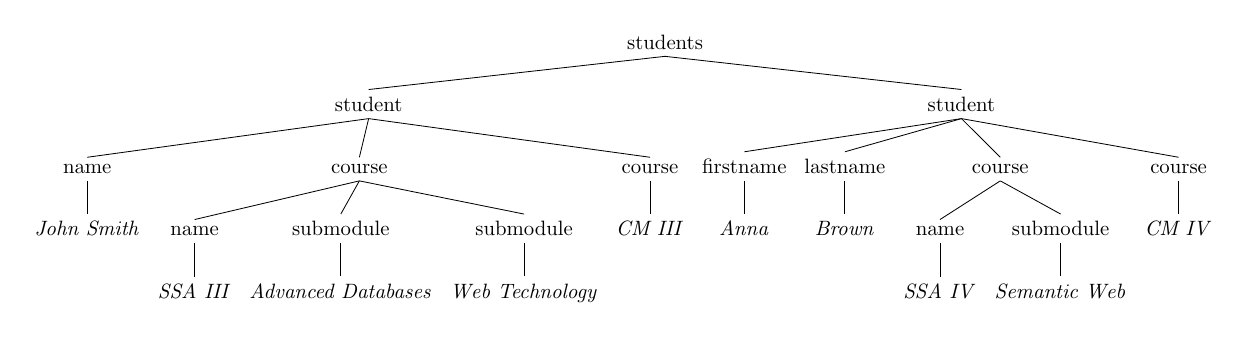
\begin{tikzpicture}[scale=.75]
\Tree[.students
	[.student 
		[.name \textit{John Smith} ]
		[.course 
			[.name \textit{SSA III} ]
			[.submodule \textit{Advanced Databases} ]
			[.submodule \textit{Web Technology} ]
		]
           [.course \textit{CM III} ]
	]
      [.student 
		[.firstname \textit{Anna} ]
		[.lastname \textit{Brown} ]
		[.course
			[.name \textit{SSA IV} ]
			[.submodule \textit{Semantic Web} ]
		]
           [.course \textit{CM IV} ]
	]
]

\end{tikzpicture}

\subsection*{b) \textit{Write a DTD for} teachers.xml.}

This DTD was validated using the \verb|lxml| Python package. The provided file, \verb|teachers.xml|, was modified slightly to facilitate this.

\begin{verbatim}

<?xml encoding="UTF-8"?>
<!ELEMENT teachers (teacher*)>
    <!ELEMENT teacher (name, course*)>
    <!ATTLIST teacher
        jobRole CDATA #REQUIRED
        joiningDate CDATA #REQUIRED>
    <!ELEMENT course (name,submodule+)>
        <!ELEMENT submodule (name,year+)>
            <!ELEMENT year (#PCDATA)>
            <!ELEMENT name (#PCDATA)>

\end{verbatim}

However, with limited examples, and no formal specification, there are ambiguities:

\begin{itemize}

\item{Should a teacher teach at least one course to be included in \verb|teachers.xml|, i.e. \verb|<!ELEMENT teacher (name, course+)>|?}
\item{Should a course contain at least one submodule to be included in \verb|teachers.xml|, i.e. \verb|<!ELEMENT course (name, submodule+)>|?}
\item{Which attributes (if any) are \verb|#REQUIRED|, \verb|#IMPLIED|, or \verb|#FIXED|? Are there default values?}
\item{Are there are limited number of values for \verb|jobRole|? If there were only two roles available, for instance, \verb|Professor| and \verb|Researcher|, the attribute declaration should be \verb|<!ATTLIST teacher jobRole(Professor| $|$ \verb|Researcher)>|.}

\end{itemize}

\subsection*{c) \textit{Is it possible to write a DTD for} \texttt{students.xml}?}

It is not possible. The difficult construct is \verb|<course>|. A student needs one or more courses (\verb|course+|) but a course can either be \verb|#PCDATA| or \verb|(name, submodule*)|, and DTD does not allow mixed delcarations such as \verb|<!ELEMENT course (#PCDATA| $|$ \verb|(name, submodule*)>|. This problem could be eliminated by forbidding \verb|#PCDATA| in \verb|<course>| and always using the \verb|<name>| element, i.e. by changing:

\begin{verbatim}

<student enrolmentDate="2016">
        <firstname>Anna</firstname>
        <lastname>Brown</lastname>
        <course>
            <name>Software, Systems and Applications IV</name>
            <submodule>Semantic Web</submodule>
        </course>
        <course>Computing Methodologies IV</course>
    </student>

\end{verbatim}

to:

\begin{verbatim}

<student enrolmentDate="2016">
        <firstname>Anna</firstname>
        <lastname>Brown</lastname>
        <course>
            <name>Software, Systems and Applications IV</name>
            <submodule>Semantic Web</submodule>
        </course>
        <course>
            <name>Computing Methodologies IV</name>
        </course>
    </student>

\end{verbatim}

The problematic DTD element would then be \verb|<!ELEMENT course (name, submodule*)>|

\clearpage

\section*{Part B}

\subsection*{a) \textit{Find all students who study "Advanced Databases" this year.}}

\begin{enumerate}

	\item{Select students for this year:} 

\begin{center}

	\verb|/students[@year='2019-2020']|

\end{center}

	\item{Select all branches with a \verb|submodule| node with a text value of 'Advanced Databases':}

\begin{center}

	\verb|/student/course/submodule[text()='Advanced Databases']|

\end{center}

	\item{Return the \verb|<student>| ancestors from the matches in step $2$:}

\begin{center}

	\verb|/ancestor::student|

\end{center}

\end{enumerate}

The output is:

\begin{verbatim}

 <student enrolmentDate="2017">
        <name>John Smith</name>
        <course>
            <name>Software, Systems and Applications III</name>
            <submodule>Advanced Databases</submodule>
            <submodule>Web Technology</submodule>
        </course>
        <course>Computing Methodologies III</course>
    </student>

\end{verbatim}

This approach is robust; there are no obvious limitations.

\subsection*{b) \textit{Find all teachers who teach "Advanced Databases" this year.}}

\begin{enumerate}

	\item{Select all \verb|submodule| branches with nodes \verb|name| and \verb|year| with values 'Advanced Databases' and '2019-2020', respectively:} 

\begin{center}

	\verb|/teachers/teacher/course/submodule[name='Advanced Databases' and year='2019-2020']|

\end{center}

	\item{Return the \verb|<teacher>| ancestors from the matches in step $1$:}

\begin{center}

	\verb|/ancestor::teachers|

\end{center}

\end{enumerate}

The output is:

\begin{verbatim}

<teacher joiningDate="2018" jobRole="Professor">
        <name>Alexandra Cristea</name>
        <course>
            <name>Software, Systems and Applications III</name>
            <submodule>
                <name>Advanced Databases</name>
                <year>2018-2019</year>
                <year>2019-2020</year>
            </submodule>
        </course>
        <course>
            <name>Software, Systems and Applications IV</name>
            <submodule>
                <name>Semantic Web</name>
                <year>2018-2019</year>
                <year>2019-2020</year>
            </submodule>
        </course>
    </teacher>

\end{verbatim}

This approach is robust; there are no obvious limitations.

\subsection*{c) \textit{How many years has Professor Cristea been teaching "Advanced Databases" (at Durham)?}}

XQUERY

\subsection*{d) \textit{Find all students in year 3 currently taught by Alexandra.}}

XQUERY

\subsection*{e) \textit{How many teachers and how many students are kept in the databases where the last name is not known?}}

XQUERY

\end{document}
